% I'm not totally sure, if this should be described together or seperate, but somehow or SCRUM approach and the Redmine
% stuff should be mentioned somewhere before the developing part and as this are probably only three pages or somethin
% it probably could be integrated here
\chapter{Project Workflow and  Requirements}\label{chap:systemRequirements}

First of all, we've got a confession to make: Unplagged is like a big playground of new 
workflows and technologies for us, as we are aiming to incorporate 
\enquote{best-practices} wherever possible, or at least what we currently consider to be best-practices. 

We believe this approach is necessary, because of the 
fact, that we are essentially trying to incubate Unplagged as a real open source project and this will 
only work if
it is well crafted and if cutting-edge workflows and technologies are used. Nearly all of the team members
are also working in some kind of web related side job, so we all got enough experiences with the problems that can 
occur during the maintenance of badly designed software.

Most of the times this works pretty well, but sometimes we are still trying to figure out how to 
get everyone up to speed with every technology and part of the system or how to divide the responsibilites carefully.

To start this project, we opted to use \textit{Scrum}\footnote{A nice introduction into Scrum is \enquote{The Scrum Primer} 
of the Scrum Alliance: \url{http://www.scrumalliance.org/resources/339}} 
as our agile development approach. If you are familiar with this
methodology, you may notice, that there could be a few problems when considering, that the team is working mostly 
distributed
without a common office and with very different time tables for each of the members.

We struggled a bit to tweak the workflow that is required by Scrum to fit the situation we faced, but you will see in the
following what we came up with.

\section{The Workflow}

To make it possible to work efficiently together in this kind of environment, we chose to use
\href{http://www.redmine.org/}{Redmine} as our project management tool, which you can access under:

\begin{itemize}
\item \url{http://tickets.unplagged.com}
\end{itemize}

If you register there, an administrator should grant you access to the tickets and the wiki, so that you can participate
in solving the problems at hand.

\begin{figure}[htbp]
  \centering
    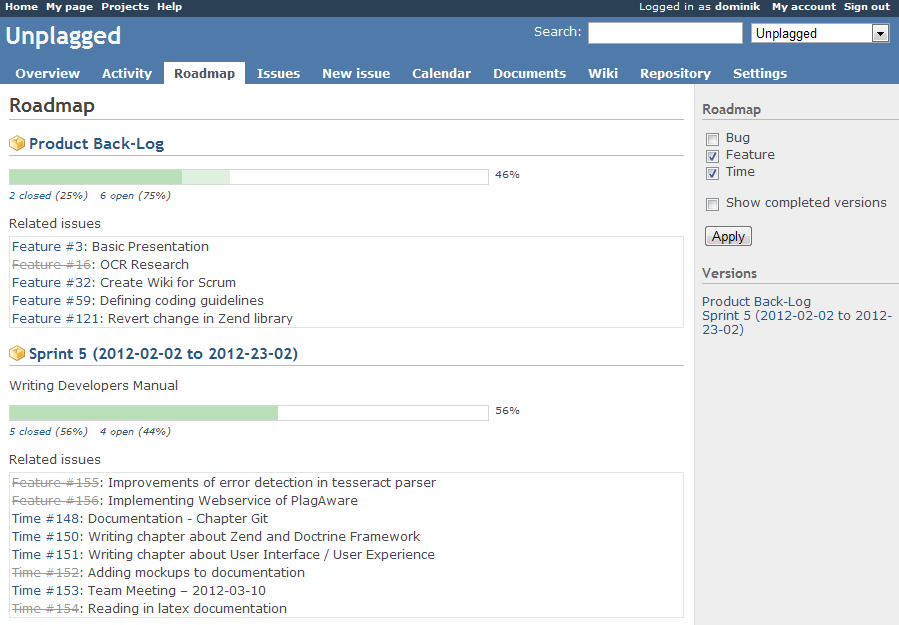
\includegraphics[width=\textwidth]{images/roadmap.png}
  \caption{Redmine Roadmap}
  \label{fig:roadmap}
\end{figure}

What we are doing there is to map every \textit{Sprint} and the \textit{Product Backlog} to Redmine's notion of \enquote{Version} and
every identified \textit{User Story} to an \enquote{Issue}.

You can see in figure \ref{fig:roadmap} the view of the roadmap, with the current sprint 5 designated to create this very
document at the bottom and a not very well filled product backlog at the top. 

Normally 
every identified user story that is not part of the current sprint should be in the product backlog (and we got plenty), 
but as we were still working
in our small group at this point, the hassle of filling in all the tickets seemed unnecessary. This is something that
will be fixed in the near future, so that you are able to see where the development is going.

Currently we are working mostly with four week long sprints, to overcome the problem that we are not working fulltime
on the tickets, which is something that scrum normally assumes. 

To have a nice statistical overview and more planning security for the \enquote{scrums}, it is required to log the time 
that was spent on an issue within redmine.

% Redmine description, Meetings, Debbie, Scrum Cards, Server, Website



\subsection{Product Owner --- \enquote{The Debbie Meetings}}


\begin{figure}[!h]
  \centering
    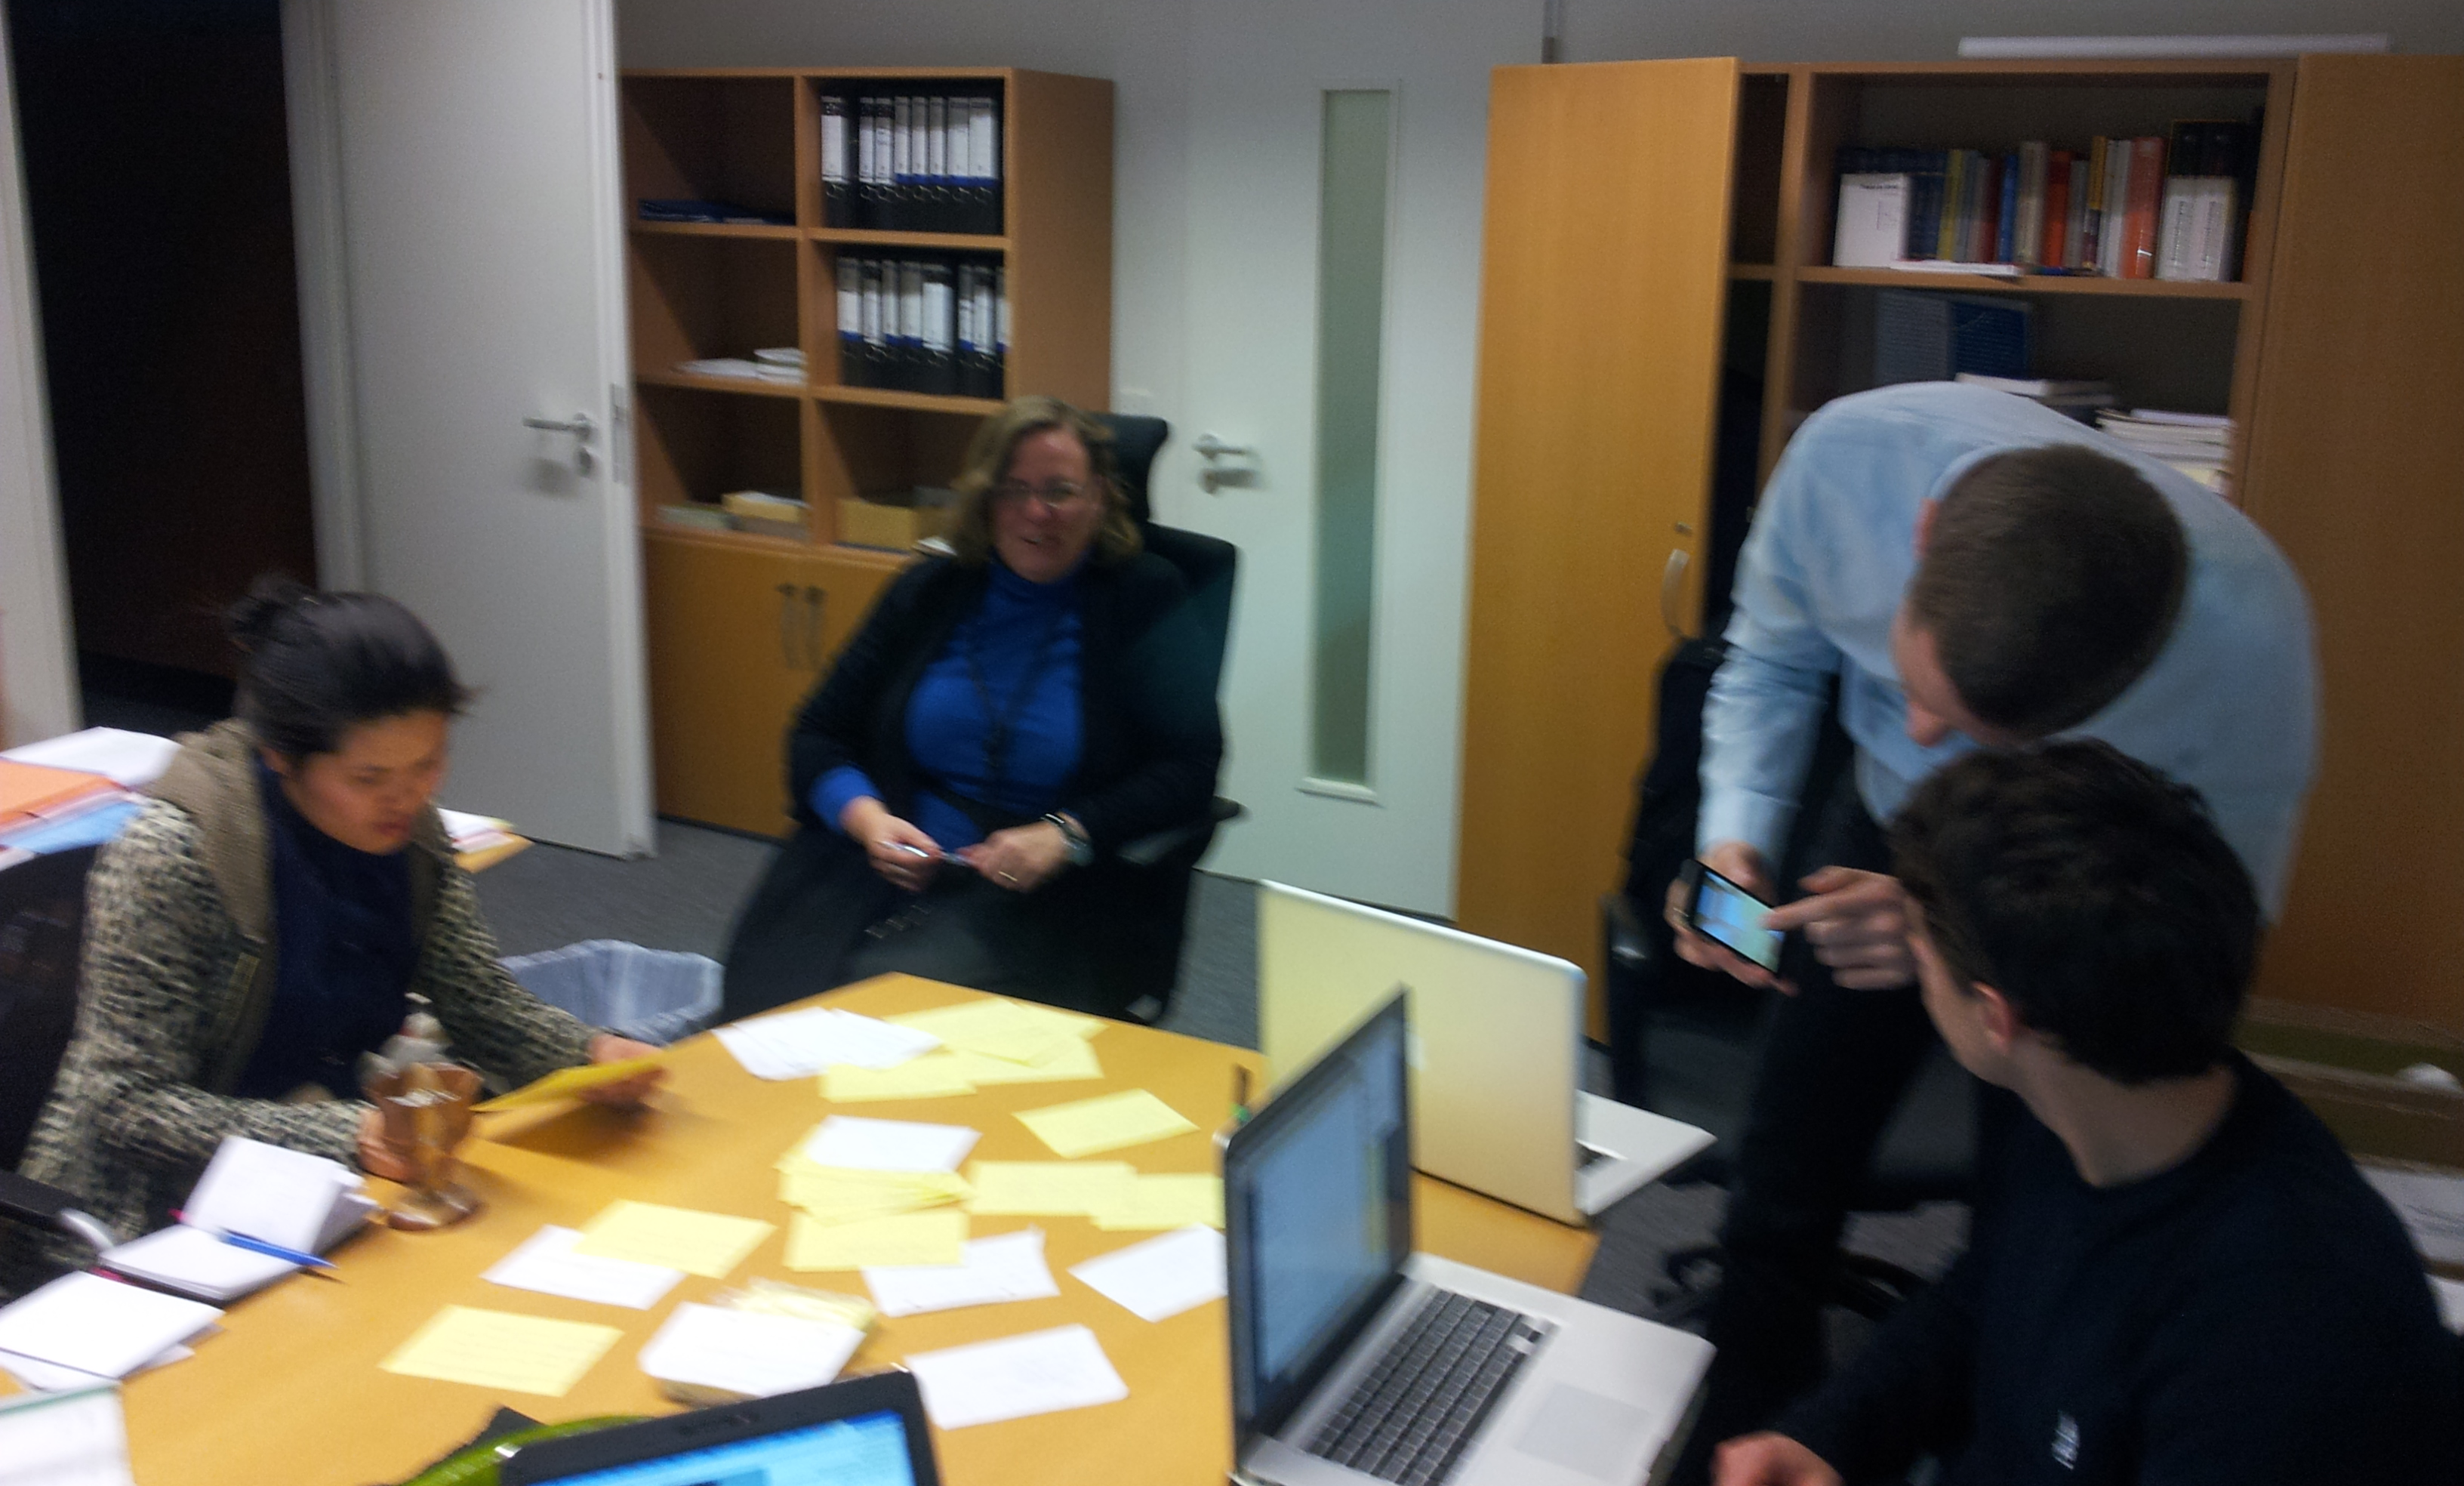
\includegraphics[width=0.8\textwidth]{images/2011-11-15-user-stories-6.jpg}
  \caption{Scrum Meeting}
  \label{fig:scrumming}
\end{figure}

To figure out the user stories we mostly rely on what we internally call \enquote{Debbie Meetings}.
Normally every two weeks, the members of the team meet with Prof. Weber-Wulff, who we state to be our \textit{Product
Owner}.

If we have a prototype that we consider to have enough business value to be shown to more people, the focus will 
probably shift away to a more broader understanding of the product owner, because there are some more sources from
which feedback on the system can be gathered.

\begin{figure}[!h]
  \centering
    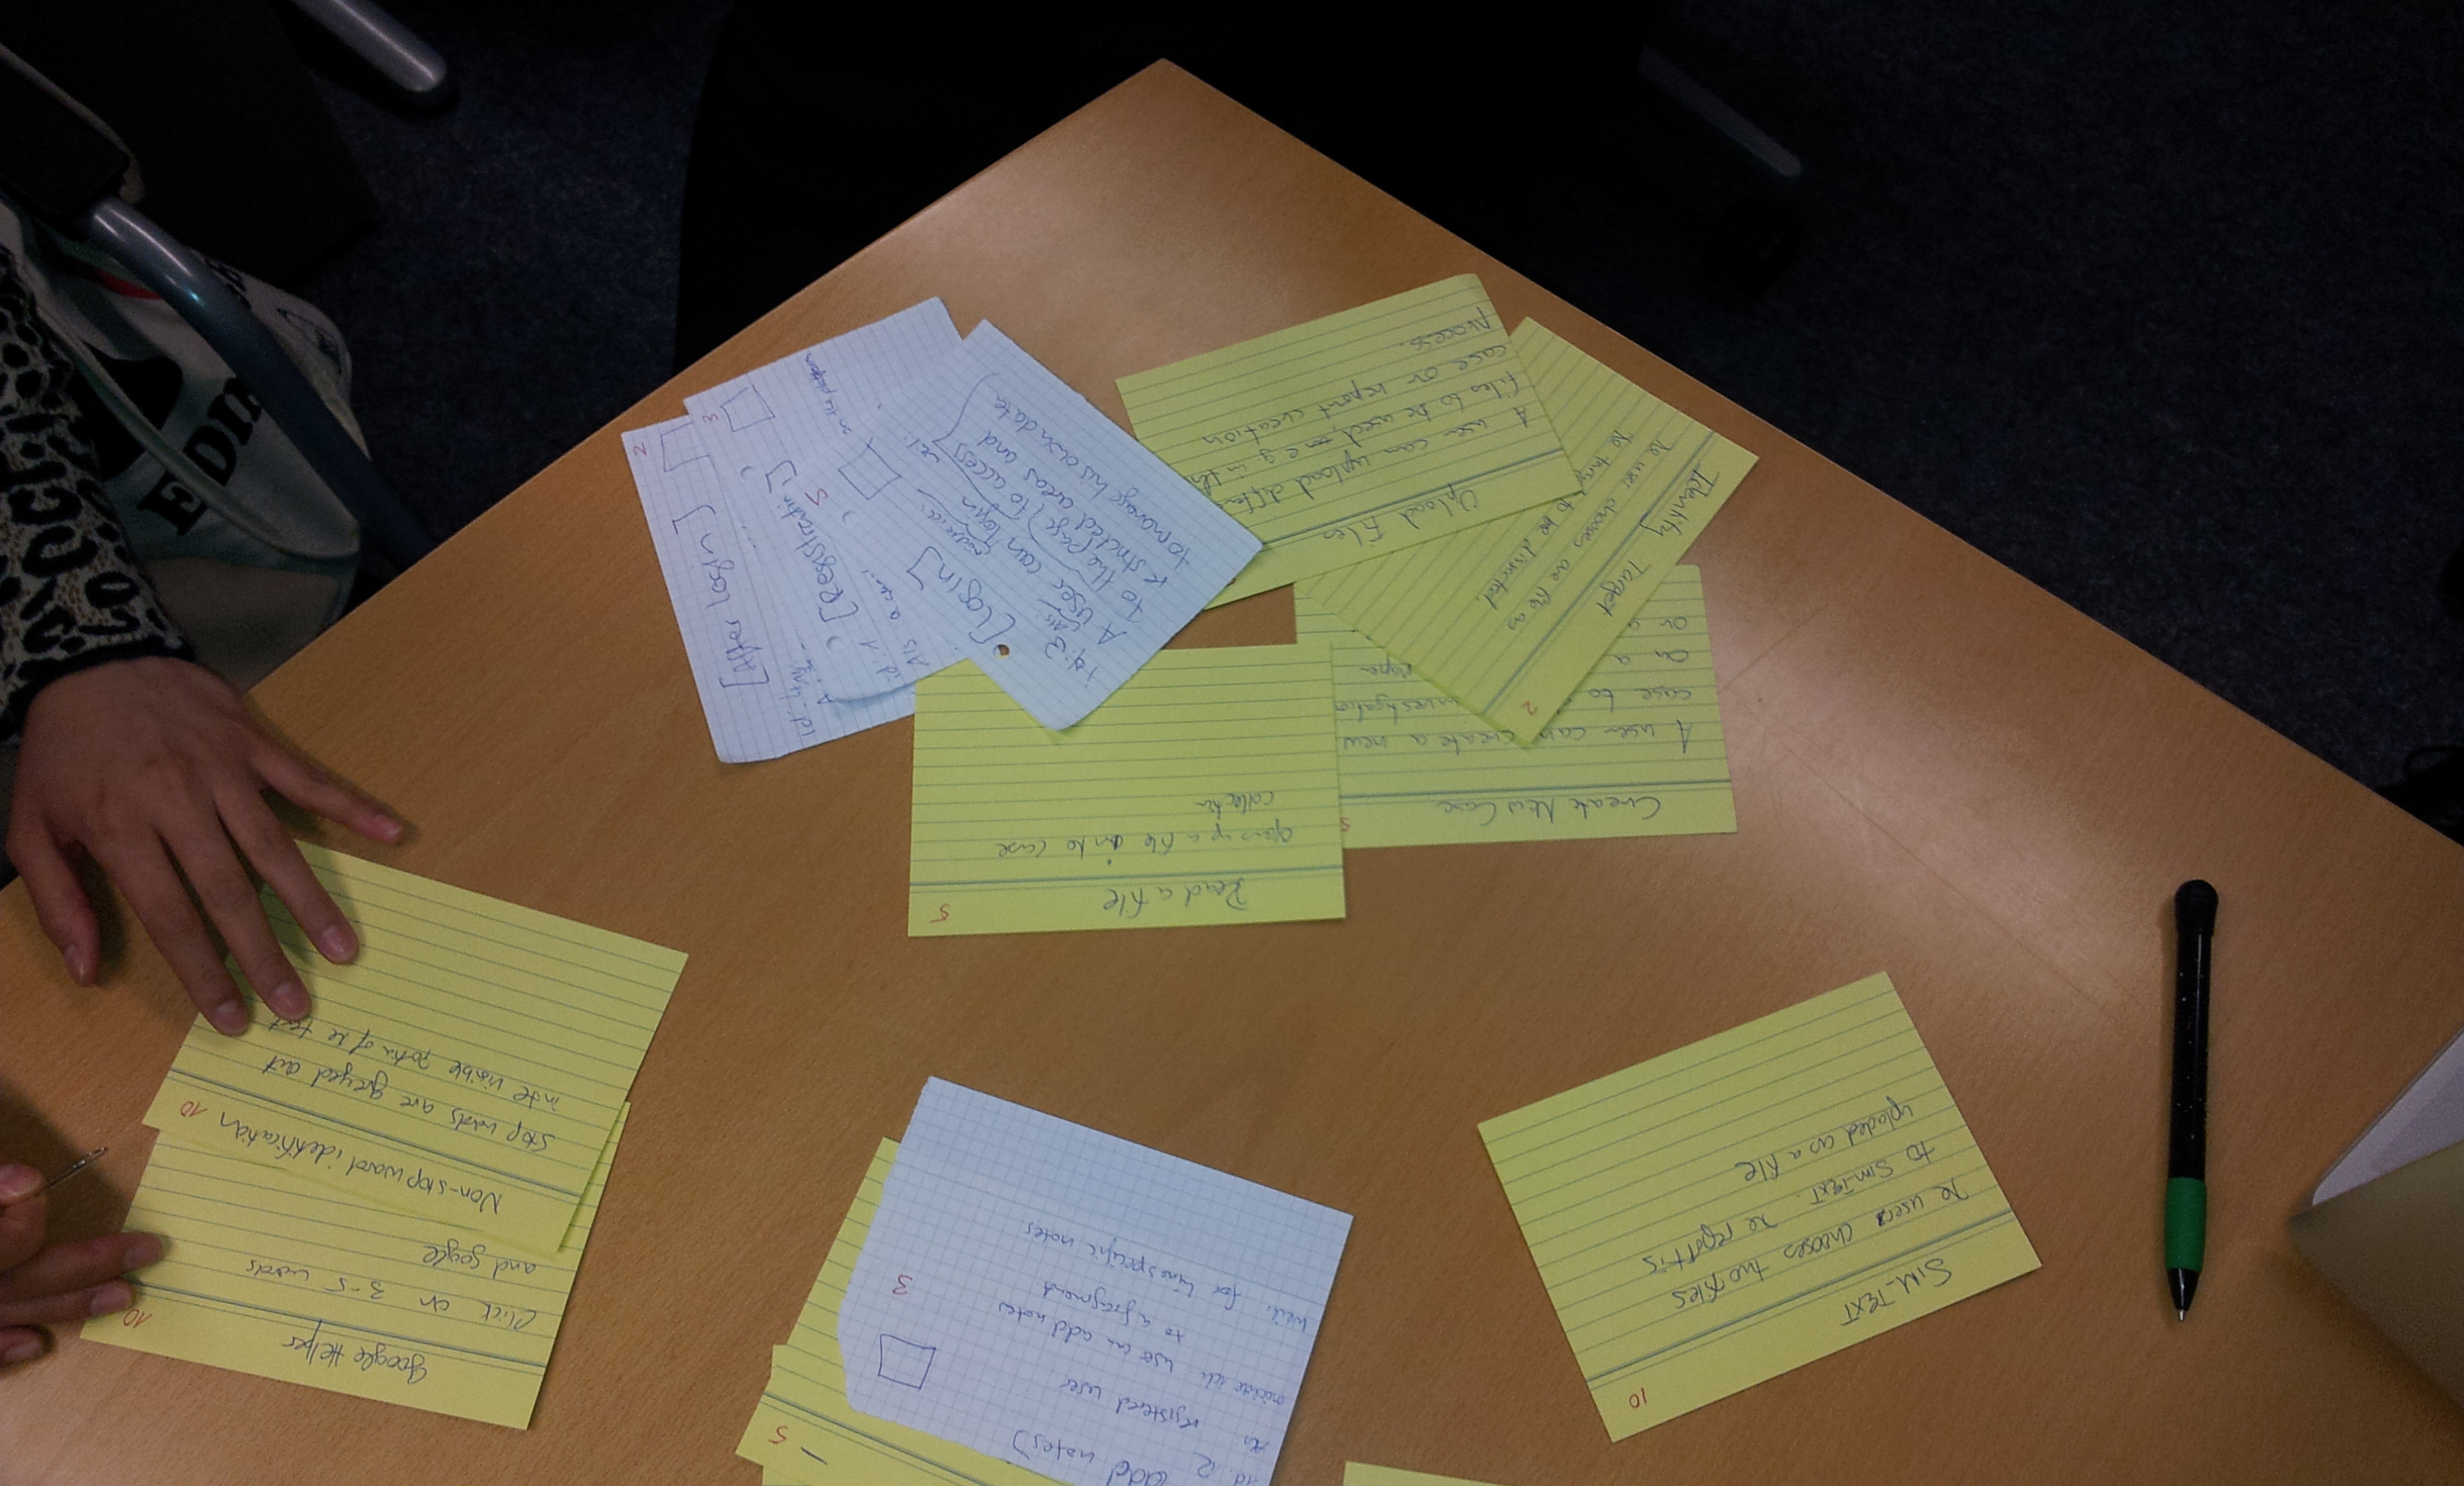
\includegraphics[width=0.8\textwidth]{images/2011-11-15-user-stories-4.jpg}
  \caption{User Stories}
  \label{fig:userStories}
\end{figure}

\subsection{Team Meetings}

The Unplagged version of the \textit{Daily Scrum} is currently a weekly meeting


\section{Target Group}

\section{User roles}
%This is copied from the wiki, so probably copy back there when the text is finished
As the Unplagged system will provide a permission based user system, our goal is to make it possible, to create custom user roles from an administration area and make it possible for users to have multiple user roles in one case and also different roles for different cases.
The standard roles which will be provided by the system are:

\begin{description}
\item[Guest]
A user without a valid login can only see the parts of cases that are set to be public.
\item[Registered]
Registered users can get \enquote{promoted} to higher roles and contribute to publicly editable cases.
%Note: Do we want users to register themselves? Or do we have just an admin, that takes care of this? I'm currently also not sure if this will really need to be a role, or if Guest and Registerd are just two basic states.
\item[Collaborator]
Collaborators are registered users who were granted access to a specific case. Collaborators can access and edit these projects.
\item[Case-Manager]
Case-Managers can set up new cases and manage colloborators for their cases and project versions. They may have the permission to add or remmove project members.
%Note: What does manage project versions mean?
\item[Admin]
An admin owns all permissions, such as user administration or project administration. They also hvae the ability to to block/unblock an existing case.
\end{description}

\section{Basic functionalities}

\section{Document Parser}

\section{Detection Modes}

\section{Plugin Architecture}

%Perhaps better on the way for every part?
\section{Use Cases}
